\documentclass[a4paper, 12pt]{article}

% Margins
\topmargin=-0.45in
\evensidemargin=0in
\oddsidemargin=0in
\textwidth=6.5in
\textheight=9.0in
\headsep=0.25in 

%package usage
\PassOptionsToPackage{svgnames}{xcolor}
\usepackage[colorlinks=true, citecolor=blue, linkcolor=purple]{hyperref}
\usepackage[english]{babel}
\usepackage[latin1]{inputenc}
\usepackage{enumitem}
\usepackage{indentfirst}
\usepackage{colortbl}
\usepackage{longtable}
\usepackage{animate}
\usepackage{threeparttablex}
\usepackage{etoolbox}
\usepackage{rotating}
\usepackage{multirow}
\usepackage{pdflscape}
\usepackage{tablefootnote}
\usepackage[table,xcdraw]{xcolor}
\usepackage{amsmath}
\usepackage{flafter} 
\usepackage{dcolumn} 
\usepackage{natbib}
\usepackage{rotating}	
\usepackage{adjustbox}
\usepackage{amsthm}
\usepackage{graphicx}
\usepackage{amssymb}
\usepackage{tcolorbox}
\usepackage{lipsum}
\usepackage{tikz}
\usepackage{tabularx}
\tcbuselibrary{skins,breakable}
\usetikzlibrary{shadings,shadows}
\usepackage{threeparttable}
\usepackage{subfig}
\usepackage{setspace}
\usepackage{booktabs}
\usepackage{placeins}
\usepackage{enumitem}
\usepackage{natbib}
\usepackage{filecontents}
\usepackage[encoding,filenameencoding=utf8,extendedchars,space]{grffile}
\newcommand{\addfig}[2]{\begin{center}
			\includegraphics[width=#1\textwidth]{#2}
	\end{center}
}

%\usepackage[capposition=top]{floatrow}
%\usepackage[colorinlistoftodos]{todonotes}
\newcommand{\expect}[2]{\mathbb{E}_{#2}\left(#1\right)}

\newtheorem{theorem}{Theorem}[section]
\newtheorem{corollary}{Corollary}[theorem]
\newtheorem{proposition}[theorem]{Proposition}

\newcommand{\alert}[1]{{\textbf{\color{red}#1}}}
%general commands

\newcommand{\bcite}{\begin{quote}}
\newcommand{\ecite}{\end{quote}}
\newcommand{\beqns}{\begin{eqnarray*}}
\newcommand{\eeqns}{\end{eqnarray*}}
\newcommand{\beqn}{\begin{eqnarray}}
\newcommand{\eeqn}{\end{eqnarray}}
\newcommand{\benu}{\begin{enumerate}}
\newcommand{\eenu}{\end{enumerate}}
\newcommand{\bitem}{\begin{itemize}}
\newcommand{\eitem}{\end{itemize}}
\newcommand{\smallGap}{\vspace{.25cm}}

\newenvironment{block}[1]{%
	\tcolorbox[beamer,%
	noparskip,breakable,
	colback=LightGreen,colframe=DarkGreen,%
	colbacklower=LimeGreen!75!LightGreen,%
	title=#1]}%
{\endtcolorbox}


\newcommand{\sym}[1]{\rlap{#1}}% Thanks David Carlisle

\usepackage{siunitx}
\sisetup{
	detect-mode,
	group-digits		= false,
	input-symbols		= ( ) [ ] - +,
	table-align-text-post	= false,
	input-signs             = ,
}

%mathematical commands
\newcommand{\problemIndustries}{(A_t\cup \Omega_t)}
\newcommand{\red}[1]{{\color{red}#1}}
\newcommand{\normalIndustries}{\problemIndustries^C}
\newcommand{\sumNormalIndustries}{\sum_{j\in\normalIndustries}}
\newcommand{\sumProblemIndustries}{\sum_{j\in\problemIndustries}}
\newcommand{\sumWithinNormal}{\sum_{j\in\normalIndustries\cap \Gamma_t}}
\newcommand{\sumWithinProblem}{\sum_{j\in\normalIndustries\cap \Gamma_t^C}}
\newcommand{\ser}[1]{s_{er#1}}
\newcommand{\cov}{\text{cov}}
\newcommand{\explain}[2]{\underbrace{#1}_{\parbox{\widthof{\ensuremath{#1}}}{\footnotesize\raggedright #2}}}
\newcommand{\lfpthresh}[1]{\underline{\chi_{#1 lt}}}
\newcommand{\crho}{\frac{\sigma-1}{\sigma}}
\newcommand{\crhoinv}{\frac{\sigma}{\sigma-1}}

\newcommand{\lquote}[3][]{\bcite #2 \citep[#1]{#3} \ecite}

\newcommand{\laquote}[3][]{\bcite #2 \citepalias[#1]{#3} \ecite}
\usepackage{tabularx}

\begin{document}

\section{Sample}
I am restricting the sample to people:
\bitem
	\item Aged 20-60.
	\item Not in the armed forces.
	\item With non-missing occupation.
	\item Non-missing educational level.
	\item At least one year of work after leaving full-time education.
\eitem

\section{Occupation cross-walks}
\bitem
	\item The occupation classification of the LFS changes every ten years.
	\item The new version of the SES/LFS provides cross-walks between the 90s - 00s - 10s classification, but the mapping is not 1-1 (e.g. some 90s codes are mapped into more than one 00s code). I address this issue as follows:
	\item \textbf{90s-00s}
	\bitem
		\item There is no cross walk available directly from the LFS. However the SES classifies observations into both the 90s and the 00s classifications.
		\item I use the SES to construct the mapping.
		\item \textbf{Issues}
		\bitem
			\item It matters at which year I look at. If I observe the SES 1997, all soc90 map into an unique soc00 category.
			\item However, when I look at 2001 the mapping is no longer unique.
			\item There are \textbf{more} soc90 codes in SES 2001 than in SES 1997.
		\eitem
		\item For now, I am using the SES 2001 to build the mapping. Main concerns with this:
		\bitem
			\item I am losing 22 jobs that were available in SES 1997.
			\item Small sample might be an issue. The main question here is: would the weights be ok?
			\item The SES 2001 gives 577 soc90-soc00 links. 31\% of those links have only 1 observation in them.
			\item 190 bsoc90 codes map uniquely into \href{https://www.dropbox.com/s/9a6xgrs32jsneuw/soc90count.txt?dl=0}{bsoc00}.
		\eitem
	\eitem
	\item \textbf{10s-00s}
	\bitem
		\item The cross walk is directly provided in the LFS.
	\eitem
\eitem

%\section{Regarding weighting}

%\bitem
%\item The dataset comes with sampling weights.
%\item According to the documentation the weights apply to people aged 20-60 years old. Even within this sample some observations in 2006 and 2012 have missing weights. The documentation does not say why this could happen. 
%\item Without weighting, the dataset has too few mean and young people.
%\item For now, all results are weighted. 
%
%\begin{table} [h!]
%	\centering
%	\caption{Share with missing weights}
%	\begin{tabular}{lccccc}
 \toprule
            &   \multicolumn{5}{c}{Year}       \\
            &        1997&        2001&        2006&        2012&       Total\\
\midrule
Share missing &         0.00&        0.00&        0.14&        0.00&        0.06\\
\bottomrule
\end{tabular}

%\end{table}
%
%
%
%\begin{center}
\begin{threeparttable}[!h]
\caption{Representativeness of the SES sample, 2006-2012}
\begin{tabular}{lccc}
\toprule
\toprule
&\multicolumn{1}{c}{(1)}&\multicolumn{1}{c}{(2)}&\multicolumn{1}{c}{(3)} \\
\textbf{Demographic}&\multicolumn{1}{c}{\textbf{Unweighted}}&\multicolumn{1}{c}{\textbf{Weighted}}&\multicolumn{1}{c}{\textbf{LFS}} \\
\midrule

\textbf{2006}\\
\midrule
Share female           	     &        0.49&        0.47 & 0.46\vspace{3mm}\\

\textit{Breakdown by age bracket}\\
\hspace{3mm}   20-29         &        0.16&        0.22& 0.22\\
\hspace{3mm}   30-39 		&        0.24&        0.25& 0.27\\
\hspace{3mm}   40-49        &        0.28&        0.27& 0.28\\
\hspace{3mm}   50-60           &        0.26&        0.23& 0.23\\
\midrule
\textbf{2012}\\
\midrule
Share female           		&        0.53&        0.46 & 0.47 \vspace{3mm}\\

\textit{Breakdown by age bracket}\\
\hspace{3mm}   20-29    	 &        0.16&        0.23& 0.23\\
\hspace{3mm}   30-39 		&        0.24&        0.25& 0.24\\
\hspace{3mm}   40-49            &        0.31&        0.28& 0.29\\
\hspace{3mm}   50-60           &        0.28&        0.24 & 0.24\\
\bottomrule
\bottomrule
\end{tabular}
\begin{tablenotes}
	\item \footnotesize{\textit{Note:} weights correspond to \texttt{weightall} variable. The third column comes from table A1 in \url{http://doc.ukdataservice.ac.uk/doc/7645/mrdoc/pdf/7645_ses_technical_briefing_may_2014.pdf}}
\end{tablenotes}
\end{threeparttable}
\end{center}

%
%
%
\begin{threeparttable}[htbp]\centering \caption{Summary statistics people with missing weights \label{sumstat}}
\begin{tabular}{l c c c c c}\hline\hline
\multicolumn{1}{c}{\textbf{Variable}} & \textbf{Mean}
 & \textbf{Std. Dev.}& \textbf{Min.} &  \textbf{Max.} & \textbf{N}\\ \hline
AGE OF RESPONDENT & 41.786 & 10.877 & 20 & 60 & 1037\\
SEX OF RESPONDENT & 0.518 & 0.5 & 0 & 1 & 1037\\
EDUCATION LEVEL HELD & 2.555 & 1.429 & 0 & 4 & 1036\\
DATASET & 2006 & 0 & 2006 & 2006 & 1037\\
\hline\end{tabular}\end{threeparttable}

%
%
%\section{Occupations to keep}
%\item Not all occupations appear in all years. It's unclear to me if this is a result of new jobs appearing, or whether this is a result of people in this occupations not being sampled.
%\item For now I restrict everything to occupations appearing in all waves.
%
%\begin{table}[h!]
%	\caption{Occupation counts}
%	\centering\begin{tabular}{lcccc} \toprule
            &\multicolumn{1}{c}{1997}&\multicolumn{1}{c}{2001}&\multicolumn{1}{c}{2006}&\multicolumn{1}{c}{2012}\\
\midrule
Number of occupations       &         180&         219&         232&         207\vspace{3mm}\\
\textit{Occupations appearing in all waves}\\
\hspace{3mm}Number of occupations     &        154 & 154& 154& 154\\
\hspace{3mm}Employment share     &        0.94&        0.92&        0.89&        0.89\\
\bottomrule
\end{tabular}

%\end{table}
%\eitem
\section{Definition of education}
\subsection{Survey of skills and employment}
\bitem
\item I am using the variable \texttt{edlev} for the education definition.
\item This variable:
\bitem
	\item Is the only variable describing education that is available in \textbf{all} years of the wave.
	\item It harmonizes the complicated UK educational classification into roughly comparable qualifications.
\eitem
\item I recover the mapping of uk qualifications into NQF levels. The levels roughly correspond to:
\bitem
	\item \textbf{Level 4+}: professional degree, bachelor's degree or more.
	\item \textbf{Level 3}: GCE A$^*$ levels / trade apprenticeship.
	\item \textbf{Level 2}: GCSE A levels.
	\item \textbf{Level 1}: GCSE D-G levels.
	\item \textbf{Level 0}: no qualification.
\eitem
\item The recovered mapping classifies correctly all \href{https://www.dropbox.com/s/jnzx818eogoiepc/educationMapping.txt?dl=0}{but 9 observations (out of 6481)}. The incorrectly classified observations probably stem from changes in the way that the ``other" category was classified.
\item The detailed mapping can be found \href{https://www.dropbox.com/s/5cutdsc5n23vqdk/educationMapping.xlsx?dl=0}{here}.
\eitem

\subsection{Labor Force Survey}
\bitem
	\item I try to reproduce the educational classification of the SES into the LFS.
	\item I match any ``new'' categories using the classification provided in the LFS 2017 documentation. See page 107 in this \href{https://www.dropbox.com/s/zk285nssot3z5dw/lfs_user_guide_vol5_classifications2009.pdf?dl=0}{pdf} 
	\item The detailed mapping can be found in the LFS sheet in this \href{https://www.dropbox.com/s/5cutdsc5n23vqdk/educationMapping.xlsx?dl=0}{document}
\eitem 	

\subsection{Grouping educational levels}
\bitem
\item I group education levels by looking at how similar the occupational distribution between them.
\item I do this by examining:
\bitem
	\item Correlation of the employment distribution across skills.
	\item Computing the pairwise Welch indexes:
	\begin{align*}
		G_{kl}&=\frac{\sum_o(q_{ko}-\bar{q}_{o})(q_{lo}-\bar{q}_{c})/\bar{q_o}}{\sqrt{(\sum_o(q_{ko}-\bar{q}_o)^2/\bar{q}_o)(\sum_o(q_{lo}-\bar{q}_o)^2/\bar{q}_o)}}
	\end{align*}
\eitem
\item The overall pattern is:
\bitem
	\item No qualification and GCSE D-G are pretty similar and they become more similar across time.
	\item Bachelor + is an independent category in its own right.
	\item	What to do with GCSE A-C and GCE A* is less clear. 
	\bitem
		\item GCSE A-C appears to be closer to No qualification and  GCSE D-G than to GCE A*.
	\eitem
\eitem
 \item At this point I do the grouping as follows:
 \bitem 
 	\item Low education: no qualification,  GCSE D-G, and  GCSE A-C.
 	\item Medium education:  GCSE A*.
 	\item High education: Bachelor +.
\eitem

% Table generated by Excel2LaTeX from sheet 'correlationLFS'
\begin{table}[htbp]
	\centering
	\caption{Welch index of the occupational distribution of employment}
	\begin{tabular}{c|rrrrr}
		& \multicolumn{1}{c}{\textbf{None}} & \multicolumn{1}{c}{\textbf{GCSE D-G}} & \multicolumn{1}{c}{\textbf{GCSE A-C}} & \multicolumn{1}{c}{\textbf{GCE A*}} & \multicolumn{1}{c}{\textbf{Bachelor's +}} \\
		\midrule
		\textbf{None} & 1.000 &       &       &       &  \\
		\textbf{GCSE D-G} & \cellcolor[rgb]{ .973,  .412,  .42}0.736 & 1.000 &       &       &  \\
		\textbf{GCSE A-C} & \cellcolor[rgb]{ .988,  .655,  .467}0.356 & \cellcolor[rgb]{ .984,  .588,  .455}0.462 & 1.000 &       &  \\
		\textbf{GCE A*} & \cellcolor[rgb]{ .965,  .91,  .514}-0.106 & \cellcolor[rgb]{ 1,  .898,  .514}-0.031 & \cellcolor[rgb]{ .992,  .745,  .486}0.215 & 1.000 &  \\
		\textbf{Bachelor's +} & \cellcolor[rgb]{ .482,  .769,  .486}-0.659 & \cellcolor[rgb]{ .424,  .753,  .482}-0.723 & \cellcolor[rgb]{ .388,  .745,  .482}-0.767 & \cellcolor[rgb]{ .627,  .812,  .494}-0.491 & 1.000 \\
	\end{tabular}%
	\caption*{\footnotesize\textit{Source:} UK LFS 1997-2017}
\end{table}%
% Table generated by Excel2LaTeX from sheet 'correlationLFS'
\begin{table}[h!]
	\centering
	\caption{Correlation of occupational distribution of employment by education level}
	\begin{tabular}{c|ccccc}
		& \textbf{None} & \textbf{GCSE D-G} & \textbf{GCSE A-C} & \textbf{GCE A*} & \textbf{Bachelor's +} \\
		\midrule
		\textbf{None} & 1.000 &       &       &       &  \\
		\textbf{GCSE D-G} & \cellcolor[rgb]{ .973,  .412,  .42}0.862 & 1.000 &       &       &  \\
		\textbf{GCSE A-C} & \cellcolor[rgb]{ .988,  .69,  .475}0.689 & \cellcolor[rgb]{ .98,  .51,  .439}0.801 & 1.000 &       &  \\
		\textbf{GCE A*} & \cellcolor[rgb]{ .918,  .898,  .51}0.481 & \cellcolor[rgb]{ .996,  .827,  .502}0.600 & \cellcolor[rgb]{ .984,  .565,  .451}0.766 & 1.000 &  \\
		\textbf{Bachelor's +} & \cellcolor[rgb]{ .388,  .745,  .482}0.078 & \cellcolor[rgb]{ .506,  .776,  .486}0.168 & \cellcolor[rgb]{ .678,  .827,  .498}0.300 & \cellcolor[rgb]{ .725,  .839,  .498}0.334 & 1.000 \\
	\end{tabular}%
	\caption*{\footnotesize\textit{Source:} UK LFS 1997-2017}
\end{table}%

\begin{center}
\begin{threeparttable}[!h]
\caption{Population by education level}
\label{tab:popcount}
\begin{tabular}{lccccc}
\toprule
\toprule
\textbf{Education level}&\multicolumn{1}{c}{\textbf{1997}}&\multicolumn{1}{c}{\textbf{2001}}&\multicolumn{1}{c}{\textbf{2006}}&\multicolumn{1}{c}{\textbf{2012}}&\multicolumn{1}{c}{\textbf{2017}} \\
\midrule
Low                 &        0.27&        0.27&        0.26&        0.25&        0.24&        0.24&        0.23&        0.22&        0.21&        0.20&        0.20&        0.20&        0.18&        0.17&        0.15&        0.14&        0.13&        0.13&        0.13&        0.13&        0.12\\
Medium              &        0.46&        0.46&        0.46&        0.46&        0.46&        0.46&        0.46&        0.46&        0.46&        0.45&        0.44&        0.45&        0.44&        0.43&        0.44&        0.44&        0.43&        0.43&        0.42&        0.41&        0.42\\
High                &        0.26&        0.28&        0.28&        0.29&        0.29&        0.30&        0.32&        0.32&        0.33&        0.35&        0.36&        0.36&        0.38&        0.40&        0.41&        0.43&        0.44&        0.44&        0.45&        0.46&        0.46\\
\midrule Total population (000)&      22,850&      23,163&      23,396&      23,706&      24,202&      24,507&      24,563&      24,835&      25,017&      25,186&      25,435&      25,354&      24,969&      25,082&      25,123&      25,474&      25,686&      26,297&      26,621&      26,834&      27,186\\
\bottomrule
\bottomrule
\end{tabular}
\begin{tablenotes}
\item \footnotesize \textit{Note:} uses data from UK LFS for the 4th quarter of each year. Table generated on 19 Jun 2020 at 11:59:20.
\end{tablenotes}
\end{threeparttable}
\end{center}

\eitem
\section{Boundary jobs}
	Let $s_{j}(o), j\in\{H,M,L\}$ denote the employment share of education level $j$ in occupation $o$. Denote as $p_i(o)$ the i-th employment share in occupation $o$, thus $p_1(o)=s_{H}(o)$ if high-education workers represent the largest share of employment in occupation $o$.
\bitem
	\item \textbf{Definition 1:} $o\in B_1$ iff:
	\beqns
	p_1(o)\leq R
	\eeqns
	\item \textbf{Definition 1:} $o\in B_2$ iff:
	\beqns
	\frac{p_1(o)}{p_1(o)+p_2(o)}\leq R
	\eeqns
	\item \textbf{Definition 3}: $o\in B_3$ iff:
	\beqns
		p_1(o)-p_2(o)\leq R-0.5
	\eeqns
	\item For any $R$, $B_3\subset B_2\subset B_1$
\eitem

\begin{figure}[h!]
	\centering
	\caption{Border under alternative definitions}
	\subfloat[Definition 1:]{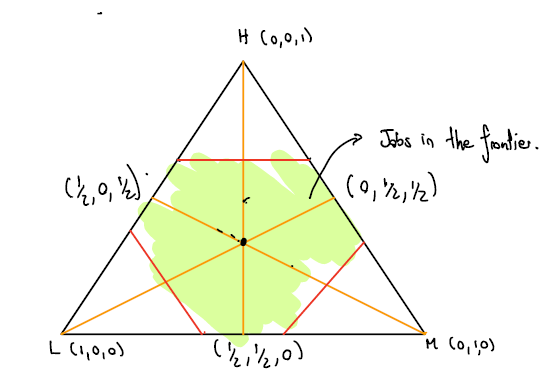
\includegraphics[width=.5\textwidth]{../output/absoluteFrontierDrawing}}
	\subfloat[Definition 2:]{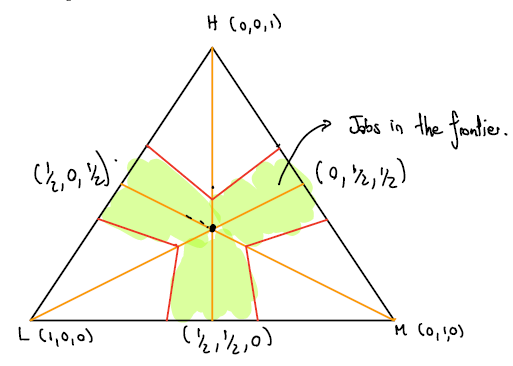
\includegraphics[width=.5\textwidth]{../output/relativeFrontierDrawing}}\\
	\subfloat[Definition 3:]{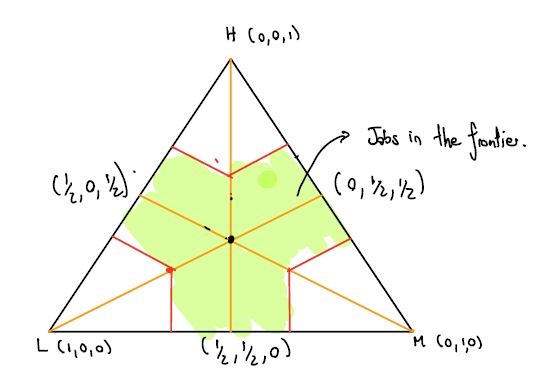
\includegraphics[width=.5\textwidth]{../output/parallelFrontierDrawing}}
\end{figure}
\newpage
\begin{figure}
	\centering
	\caption{Job classification under different boundary definitions  ($R=60\%$)}
	\subfloat[Definition 1]{\includegraphics[width=.6\textwidth]{../output/lfsBoundary160}}\\
	\subfloat[Definition 2]{\includegraphics[width=.6\textwidth]{../output/lfsBoundary260}}\\
	\subfloat[Definition 3]{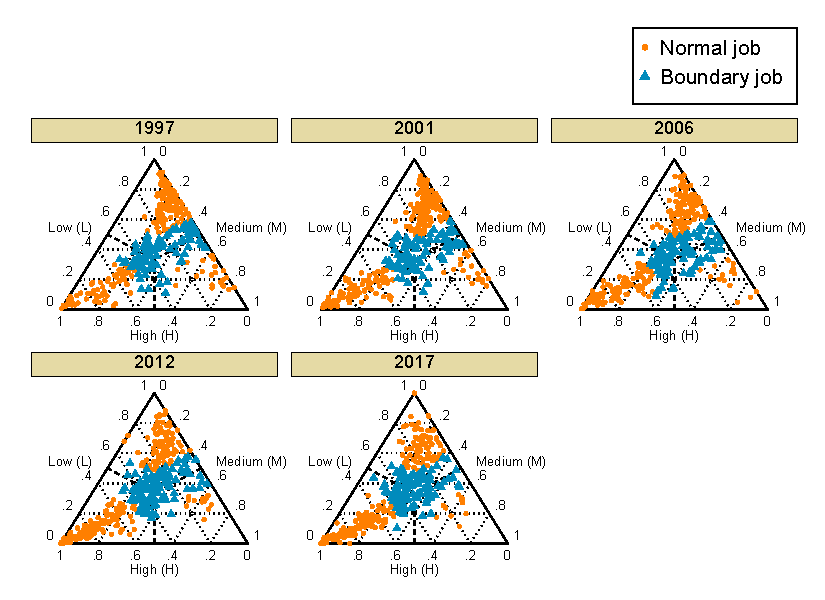
\includegraphics[width=.6\textwidth]{../output/lfsBoundary360}}
\end{figure}
\newpage 

\begin{center}
\begin{threeparttable}[!h]
\caption{Definition 1: share of occupations in the boundary}
\label{tab:shareBound}
\begin{tabular}{lccccc}
\toprule
\toprule
\textbf{Boundary threshold}&\multicolumn{1}{c}{\textbf{1997}}&\multicolumn{1}{c}{\textbf{2001}}&\multicolumn{1}{c}{\textbf{2006}}&\multicolumn{1}{c}{\textbf{2012}}&\multicolumn{1}{c}{\textbf{2017}} \\
\midrule
55\%        &        0.33&        0.33&        0.38&        0.39&        0.40\\
60\%        &        0.43&        0.45&        0.48&        0.49&        0.49\\
65\%        &        0.55&        0.54&        0.57&        0.60&        0.59\\
70\%        &        0.67&        0.64&        0.67&        0.69&        0.70\\
\midrule Observations&         332&         332&         332&         332&         332\\
\bottomrule
\bottomrule
\end{tabular}
\begin{tablenotes}
\item\footnotesize\textit{Note:} Source: UK Quarterly LFS. Table generated on  4 Jan 2020 at 15:35:28.
\end{tablenotes}
\end{threeparttable}
\end{center}

\begin{center}
\begin{threeparttable}[!h]
\caption{Definition 2: share of occupations in the boundary}
\label{tab:shareBound}
\begin{tabular}{lccccc}
\toprule
\toprule
\textbf{Boundary threshold}&\multicolumn{1}{c}{\textbf{1997}}&\multicolumn{1}{c}{\textbf{2001}}&\multicolumn{1}{c}{\textbf{2006}}&\multicolumn{1}{c}{\textbf{2012}}&\multicolumn{1}{c}{\textbf{2017}} \\
\midrule
55\%        &        0.10&        0.12&        0.10&        0.13&        0.10\\
60\%        &        0.22&        0.23&        0.23&        0.27&        0.27\\
65\%        &        0.36&        0.33&        0.35&        0.38&        0.39\\
70\%        &        0.45&        0.47&        0.48&        0.50&        0.49\\
\midrule Observations&         332&         332&         332&         332&         332\\
\bottomrule
\bottomrule
\end{tabular}
\begin{tablenotes}
\item\footnotesize\textit{Note:} Source: UK Quarterly LFS. Table generated on  4 Jan 2020 at 15:35:32.
\end{tablenotes}
\end{threeparttable}
\end{center}

\begin{center}
\begin{threeparttable}[!h]
\caption{Definition 3: share of occupations in the boundary}
\label{tab:shareBound}
\begin{tabular}{lccccc}
\toprule
\toprule
\textbf{Boundary threshold}&\multicolumn{1}{c}{\textbf{1997}}&\multicolumn{1}{c}{\textbf{2001}}&\multicolumn{1}{c}{\textbf{2006}}&\multicolumn{1}{c}{\textbf{2012}}&\multicolumn{1}{c}{\textbf{2017}} \\
\midrule
55\%        &        0.12&        0.14&        0.14&        0.16&        0.16\\
60\%        &        0.28&        0.27&        0.29&        0.32&        0.32\\
65\%        &        0.39&        0.42&        0.44&        0.44&        0.44\\
70\%        &        0.55&        0.54&        0.55&        0.57&        0.56\\
\midrule Observations&         332&         332&         332&         332&         332\\
\bottomrule
\bottomrule
\end{tabular}
\begin{tablenotes}
\item\footnotesize\textit{Note:} Source: UK Quarterly LFS. Table generated on 13 Jan 2020 at 13:02:19.
\end{tablenotes}
\end{threeparttable}
\end{center}


\subsection{Jobs by education-pair border}	
\begin{center}
\begin{threeparttable}[!h]
\caption{Definition 1: number of occupations by boundary type}
\label{tab:shareBound}
\begin{tabular}{lccccc}
\toprule
\toprule
\textbf{Boundary threshold}&\multicolumn{1}{c}{\textbf{1997}}&\multicolumn{1}{c}{\textbf{2001}}&\multicolumn{1}{c}{\textbf{2006}}&\multicolumn{1}{c}{\textbf{2012}}&\multicolumn{1}{c}{\textbf{2017}} \\
\midrule
Low-Mid     &          63&          77&          75&          76&          62\\
Mid-High    &          26&          30&          27&          31&          34\\
Low-High    &          54&          41&          58&          57&          67\\
\bottomrule
\bottomrule
\end{tabular}
\begin{tablenotes}
\item\footnotesize\textit{Note:} Source: UK Quarterly LFS. Table generated on  4 Jan 2020 at 15:35:28.
\end{tablenotes}
\end{threeparttable}
\end{center}

\begin{center}
\begin{threeparttable}[!h]
\caption{Definition 2: number of occupations by boundary type}
\label{tab:shareBound}
\begin{tabular}{lccccc}
\toprule
\toprule
\textbf{Boundary threshold}&\multicolumn{1}{c}{\textbf{1997}}&\multicolumn{1}{c}{\textbf{2001}}&\multicolumn{1}{c}{\textbf{2006}}&\multicolumn{1}{c}{\textbf{2012}}&\multicolumn{1}{c}{\textbf{2017}} \\
\midrule
Low-Mid     &          33&          39&          36&          42&          31\\
Mid-High    &          14&          15&          12&          19&          15\\
Low-High    &          25&          21&          30&          28&          42\\
\bottomrule
\bottomrule
\end{tabular}
\begin{tablenotes}
\item\footnotesize\textit{Note:} Source: UK Quarterly LFS. Table generated on  4 Jan 2020 at 15:35:32.
\end{tablenotes}
\end{threeparttable}
\end{center}

\begin{center}
\begin{threeparttable}[!h]
\caption{Definition 3: number of occupations by boundary type}
\label{tab:shareBound}
\begin{tabular}{lccccc}
\toprule
\toprule
\textbf{Boundary threshold}&\multicolumn{1}{c}{\textbf{1997}}&\multicolumn{1}{c}{\textbf{2001}}&\multicolumn{1}{c}{\textbf{2006}}&\multicolumn{1}{c}{\textbf{2012}}&\multicolumn{1}{c}{\textbf{2017}} \\
\midrule
Low-Mid     &          41&          42&          43&          51&          35\\
Mid-High    &          17&          18&          18&          21&          23\\
Low-High    &          34&          28&          35&          35&          49\\
\bottomrule
\bottomrule
\end{tabular}
\begin{tablenotes}
\item\footnotesize\textit{Note:} Source: UK Quarterly LFS. Table generated on 13 Jan 2020 at 13:02:20.
\end{tablenotes}
\end{threeparttable}
\end{center}


\subsection{Time in the border}
\begin{table}[h!]
	\caption{Definition 1: number of years in the border}
	\centering
	\begin{tabular}{lr}
	\toprule
Number of years & Number of jobs \\
\midrule
0&88 \\
1&49 \\
2&40 \\
3&41 \\
4&44 \\
5&70 \\
Total&332 \\
\bottomrule
\end{tabular}
\end{table}

\begin{table}[h!]
	\caption{Definition 2: number of years in the border}
	\centering
	\begin{tabular}{lr}
	\toprule
Number of years & Number of jobs \\
\midrule
0&156 \\
1&55 \\
2&56 \\
3&35 \\
4&20 \\
5&10 \\
Total&332 \\
\bottomrule
\end{tabular}
\end{table}

\begin{table}[h!]
	\caption{Definition 3: number of years in the border}
	\centering
	\begin{tabular}{lr}
	\toprule
Number of years & Number of jobs \\
\midrule
0&138 \\
1&53 \\
2&57 \\
3&35 \\
4&27 \\
5&22 \\
Total&332 \\
\bottomrule
\end{tabular}
\end{table}


\subsection{Border jobs examples}
\input{../output/borderExamples1.tex}
\input{../output/borderExamples2.tex}
\input{../output/borderExamples3.tex}

\section{Going back to SES}
\bitem
	\item I have 192 out of 332 occupations which I can track throughout the whole period.
	\item Occupations appearing only 4 times across the period could be an issue. They account for about 25\% of employment in the \href{https://www.dropbox.com/s/bzkjsuhid0z5yaf/sesPanelEmpshare.txt?dl=0}{LFS}.
	\bitem 
		\item Out of these: those not appearing in 1997 are the issue. They account for about 22\% of total employment in the LFS.
		\item Those that are missing in a year other than 1997 are probably just due to sampling. They are fairly small so I am very confident excluding them.
	\eitem
	\item Missing occupations after 1997 are probably the result of sampling error. They are generally small and account at most for 2\% of LFS employment.
	\item Crux of the issues are in the change between 1997 and 2001.
\eitem
\end{document}

